\documentclass{beamer}

% --- Metropolis theme (modern, minimal) ---
\usetheme{metropolis}
\usepackage{appendixnumberbeamer}

\usepackage{xcolor}
\usepackage{mathrsfs}
\usepackage{amsmath}
\usepackage{amssymb}
\usepackage{booktabs}
\usepackage{hyperref}
\usepackage{caption}
\usepackage{graphicx}
\usepackage{subcaption}
\usepackage{tikz}
\usetikzlibrary{shapes.geometric, arrows.meta, positioning, fit, backgrounds}
\usepackage{tcolorbox}
\tcbuselibrary{skins, breakable}
\captionsetup[figure]{font=tiny}
\graphicspath{{../../results/}}

\usepackage[
    backend=biber,
    style=alphabetic,
    sorting=ynt
]{biblatex}
\addbibresource{bibliography.bib}

% --- Colour palette ---
\definecolor{CSred}{RGB}{160,32,60}
\definecolor{CSgrey}{RGB}{136,121,150}
\definecolor{CSlight}{RGB}{245,240,248}
\definecolor{alertorange}{RGB}{200,80,0}
\definecolor{metrobg}{RGB}{250,249,252}

% --- Metropolis overrides ---
\setbeamercolor{normal text}{fg=black!85, bg=metrobg}
\setbeamercolor{frametitle}{bg=CSred, fg=white}
\setbeamercolor{title separator}{fg=CSred}
\setbeamercolor{progress bar}{fg=CSred, bg=CSgrey!40}
\setbeamercolor{alerted text}{fg=CSred}
\setbeamercolor{block title}{bg=CSred, fg=white}
\setbeamercolor{block body}{bg=CSlight}
\metroset{progressbar=frametitle, sectionpage=none, numbering=fraction}
\setbeamerfont{frametitle}{series=\bfseries, size=\normalsize}

% --- tcolorbox styles ---
\tcbset{
  keybox/.style={
    colback=CSlight, colframe=CSred, fonttitle=\bfseries\small,
    boxrule=0.8pt, arc=3pt, left=5pt, right=5pt, top=4pt, bottom=4pt
  },
  warnbox/.style={
    colback=orange!7, colframe=alertorange, fonttitle=\bfseries\small,
    boxrule=0.8pt, arc=3pt, left=5pt, right=5pt, top=4pt, bottom=4pt
  },
  stressbox/.style={
    colback=CSlight, colframe=CSgrey, fonttitle=\bfseries\footnotesize,
    boxrule=0.8pt, arc=4pt, left=4pt, right=4pt, top=3pt, bottom=3pt
  } 
}

% --- Title info ---
\title{The No-U-Turn Sampler}
\subtitle{Adaptively Setting Path Lengths in Hamiltonian Monte Carlo}
\author{Adonis Jamal \quad Jean-Vincent Martini}
\institute{\'Ecole Normale Sup\'erieure Paris-Saclay --- MVA 2025--2026}
\date{March 12, 2026}

\titlegraphic{%
  \hfill
  
\includegraphics[height=1.0cm]{img/logo_ens-ps.png}
  \hspace{0.4cm}
  
\includegraphics[height=1.1cm]{img/logo_mva.jpg}
}

\begin{document}

\maketitle

% ==============================================================================
% SECTION 1: MOTIVATION
% ==============================================================================
\begin{frame}{MCMC \& Hamiltonian Monte Carlo}
    \textbf{The challenge}
    \begin{itemize}
        \item Exact posterior inference is often intractable.
        \item MCMC is asymptotically unbiased and broadly applicable \cite{neal1993probabilistic}.
        \item Random-walk \& Gibbs \cite{metropolis1953equation,geman1984stochastic} struggle in high-dimensional or correlated spaces.
    \end{itemize}

    \begin{tcolorbox}[keybox, title=Hamiltonian Monte Carlo]
        Auxiliary momentum $r \!\sim\! \mathcal{N}(0,I)$\,+\,leapfrog
        \[p(\theta,r)\!\propto\!\exp\!\left\{\mathcal{L}(\theta)-\tfrac{1}{2}r^\top r\right\}\]
        Volume-preserving means proposals can be \textbf{distant} yet \textbf{highly probable}.
    \end{tcolorbox}
\end{frame}

\begin{frame}{The HMC Tuning Problem}
  \noindent
  \begin{minipage}[t]{0.49\textwidth}
    \begin{tcolorbox}[warnbox, title=Step size $\varepsilon$, height=2.8cm]
      \small
      Too small $\Rightarrow$ wasted computation\\[3pt]
      Too large $\Rightarrow$ high rejection rate
    \end{tcolorbox}
  \end{minipage}
  \hfill
  \begin{minipage}[t]{0.49\textwidth}
    \begin{tcolorbox}[warnbox, title=Leapfrog steps $L$, height=2.8cm]
      \small
      Too small $\Rightarrow$ random walk behaviour\\[3pt]
      Too large $\Rightarrow$ trajectory loops back
    \end{tcolorbox}
  \end{minipage}

  \vspace{0.2cm}
  Good $L$ requires costly preliminary runs and expert knowledge, a key barrier to adoption.

  \vspace{0.2cm}
  \begin{tcolorbox}[keybox, title=NUTS addresses both \cite{main}]
    \begin{itemize}
      \item \textbf{Adaptive $L$:} No-U-Turn criterion stops when trajectory doubles back.
      \item \textbf{Adaptive $\varepsilon$:} Dual averaging during warm-up \cite{nesterov2009primal}.
    \end{itemize}
  \end{tcolorbox}
\end{frame}

% ==============================================================================
% SECTION 2: NUTS METHODOLOGY
% ==============================================================================
\begin{frame}{The No-U-Turn Criterion}
  \textbf{Key idea:} Stop when further steps move the proposal \emph{back} towards the start.

  \vspace{0.2cm}
  Monitor $\tfrac{d}{dt}\tfrac{1}{2}\|\tilde\theta - \theta\|^2$: when negative, the trajectory is doubling back.

  \vspace{0.15cm}
  \begin{tcolorbox}[keybox, title={U-turn condition on leaves $(\theta^-,r^-)$, $(\theta^+,r^+)$}]
    \[(\theta^+ - \theta^-)\cdot r^- < 0 \quad\text{or}\quad (\theta^+ - \theta^-)\cdot r^+ < 0\]
  \end{tcolorbox}

  \vspace{0.2cm}
  Naive rule $\Rightarrow$ breaks time-reversibility. NUTS instead builds trajectories \textbf{forwards and backwards} via recursive doubling, augmented with a slice variable:
  \[u \sim \mathrm{Uniform}\!\left([0,\exp\{\mathcal{L}(\theta)-\tfrac{1}{2}r\cdot r\}]\right)\]
\end{frame}

\begin{frame}{Recursive Doubling \& Efficient Kernel}
    \textbf{Trajectory construction}
    \begin{enumerate}
      \item Draw $v_j \sim \mathrm{Uniform}(\{-1,+1\})$
      \item Take $2^j$ leapfrog steps of size $v_j\varepsilon$
      \item Grow balanced binary tree of states
      \item Halt on U-turn or instability
    \end{enumerate}
    States from a halting step are excluded from $\mathcal{C}$ to preserve detailed balance.

    \begin{tcolorbox}[keybox, title={Memory: $\mathcal{O}(2^j)\to\mathcal{O}(j)$}]
      Partition $\mathcal{C} = \mathcal{C}^{\mathrm{old}} \cup \mathcal{C}^{\mathrm{new}}$ then propose $w'\!\in\!\mathcal{C}^{\mathrm{new}}$, accept with:
      \[\min\!\left(1,\frac{|\mathcal{C}^{\mathrm{new}}|}{|\mathcal{C}^{\mathrm{old}}|}\right)\]
      Satisfies detailed balance w.r.t.\ uniform over $\mathcal{C}$.
    \end{tcolorbox}
\end{frame}

\begin{frame}{Adaptive Step Size: Dual Averaging}
  During warm-up only, drive acceptance towards target $\delta$:
  \[
    x_{t+1} = \mu - \frac{\sqrt{t}}{\gamma(t+t_0)}\sum_{i=1}^{t}H_i,
    \qquad
    \bar{x}_{t+1} = t^{-\kappa}x_{t+1} + (1-t^{-\kappa})\bar{x}_t
  \]
  \vspace{-0.1cm}
  \begin{itemize}
    \item $x=\log\varepsilon$, \quad $\mu=\log(10\varepsilon_0)$ encourages larger step sizes
    \item Fixed hyperparameters: $\gamma=0.05$,\; $t_0=10$,\; $\kappa=0.75$
  \end{itemize}

  \vspace{0.2cm}
  \begin{tcolorbox}[keybox]
    No-U-Turn criterion + dual averaging $\Rightarrow$ NUTS is \textbf{entirely tuning-free}.
  \end{tcolorbox}
\end{frame}

% ==============================================================================
% SECTION 3: OUR THEORETICAL CONTRIBUTIONS
% ==============================================================================
% \begin{frame}{Our Theoretical Contributions}
%   The original paper leaves two key results only sketched. We provide complete proofs.
% 
%   \vspace{0.2cm}
%   \begin{tcolorbox}[keybox, title={1. Uniform distribution over $\mathcal{C}$}]
%     \small From the augmented density and conditions C.1--C.4:
%     \[p(w\mid u,\mathcal{B},\mathcal{C},\varepsilon) = \frac{1}{|\mathcal{C}|}\,\mathbf{1}[w\!\in\!\mathcal{C}]\]
%     Explicit use of volume preservation (C.1) and equal generation probability (C.4).
%   \end{tcolorbox}
% 
%   \vspace{0.2cm}
%   \begin{tcolorbox}[keybox, title={2. Detailed balance of the memory-efficient kernel}]
%     \small For $w\!\in\!\mathcal{C}^{\mathrm{old}}$, $w'\!\in\!\mathcal{C}^{\mathrm{new}}$, the condition
%     $p(w|\mathcal{C})\,T(w'|w,\mathcal{C}) = p(w'|\mathcal{C})\,T(w|w',\mathcal{C})$
%     reduces to $\min(|\mathcal{C}^{\mathrm{old}}|,|\mathcal{C}^{\mathrm{new}}|) = \min(|\mathcal{C}^{\mathrm{new}}|,|\mathcal{C}^{\mathrm{old}}|)$.\;\checkmark
%   \end{tcolorbox}
% \end{frame}

\begin{frame}{The Transition Kernel \& Detailed Balance}
    To reduce memory from $\mathcal{O}(2^j)$ to $\mathcal{O}(j)$, NUTS partitions the candidate set: $\mathcal{C} = \mathcal{C}^{\text{old}} \cup \mathcal{C}^{\text{new}}$.

    \vspace{0.03cm}
    \textbf{The Proposal:}
    \begin{itemize}
        \item From state $w \in \mathcal{C}^{\text{old}}$, propose a jump to $w' \in \mathcal{C}^{\text{new}}$ uniformly.
        \item Accept with probability: $\min\left(1, \frac{|\mathcal{C}^{\text{new}}|}{|\mathcal{C}^{\text{old}}|}\right)$
    \end{itemize}

    \vspace{0.03cm}
    \begin{tcolorbox}[colback=CSlight, colframe=CSgrey, title=Proof of Detailed Balance (Intuition)]
        We must satisfy: $p(w|\mathcal{C})T(w'|w, \mathcal{C}) = p(w'|\mathcal{C})T(w|w', \mathcal{C})$
        
        \vspace{0.05cm}
        Substituting the prior $p(w|\mathcal{C}) = \frac{1}{|\mathcal{C}|}$ and the acceptance rates:
        $$ \frac{1}{|\mathcal{C}||\mathcal{C}^{\text{new}}|} \min\left(1, \frac{|\mathcal{C}^{\text{new}}|}{|\mathcal{C}^{\text{old}}|}\right) = \frac{1}{|\mathcal{C}||\mathcal{C}^{\text{old}}|} \min\left(1, \frac{|\mathcal{C}^{\text{old}}|}{|\mathcal{C}^{\text{new}}|}\right) $$
        Proving the kernel preserves the target distribution.
    \end{tcolorbox}
\end{frame}

% ==============================================================================
% SECTION 4: IMPLEMENTATION AND BENCHMARKS
% ==============================================================================
\begin{frame}{Evaluating NUTS: The Paper's Benchmarks}
    The paper tests NUTS on four targets spanning low to very high dimensions, measuring \textbf{minimum ESS per gradient evaluation} across all dimensions.

    \vspace{0.2cm}
    \noindent
    \begin{minipage}[t]{0.22\textwidth}\centering
      \begin{tcolorbox}[stressbox, title=250-D, halign=center]
        \footnotesize Multivariate Normal
      \end{tcolorbox}
    \end{minipage}
    \hfill
    \begin{minipage}[t]{0.22\textwidth}\centering
      \begin{tcolorbox}[stressbox, title=25-D, halign=center]
        \footnotesize Logistic Regression
      \end{tcolorbox}
    \end{minipage}
    \hfill
    \begin{minipage}[t]{0.22\textwidth}\centering
      \begin{tcolorbox}[stressbox, title=302-D, halign=center]
        \footnotesize Hierarchical LR
      \end{tcolorbox}
    \end{minipage}
    \hfill
    \begin{minipage}[t]{0.22\textwidth}\centering
      \begin{tcolorbox}[stressbox, title=3001-D, halign=center]
        \footnotesize Stochastic Volatility
      \end{tcolorbox}
    \end{minipage}

    \vspace{0.3cm}
    \begin{tcolorbox}[keybox]
      NUTS matches or exceeds best-tuned HMC on \textbf{all four benchmarks} without
      any trajectory-length tuning, up to $2\times$ on the Gaussian and $1.5\times$ on the
      stochastic volatility model.
    \end{tcolorbox}

    \vspace{0.15cm}
    But all four targets are \textbf{unimodal or mildly structured}. How does NUTS fare on posteriors with genuinely complex geometry?
\end{frame}


% ==============================================================================
% SECTION 5: STRESS TESTS
% ==============================================================================
\begin{frame}{Beyond the Paper: Three Stress Tests}

  \vspace{0.1cm}
  We probe three failure modes of HMC that are absent from the original evaluation:

  \vspace{0.3cm}
  % TikZ diagram of three pathologies
  \begin{center}
  \begin{tikzpicture}[>=Stealth, font=\small]

    % Box 1: Multimodality
    \node[draw=CSred, fill=CSlight, rounded corners=4pt, inner sep=6pt,
          text width=2.6cm, align=center] (A) {
      \textbf{Multimodality}\\[3pt]
      \begin{tikzpicture}[scale=0.38]
        \fill[CSred!70] (-2.4, 0) ellipse (0.28 and 0.6);
        \fill[CSred!70] (0,    0) ellipse (0.28 and 0.6);
        \fill[CSred!70] (2.4,  0) ellipse (0.28 and 0.6);
        \draw[->, gray, thin] (-3.1,0) -- (3.1,0);
      \end{tikzpicture}\\[2pt]
      {\footnotesize BNN, 191-D\\$5!\!\times\!5!=14400$ modes}
    };

    % Box 2: Dense correlations
    \node[draw=CSred, fill=CSlight, rounded corners=4pt, inner sep=6pt,
          text width=3.2cm, align=center, right=0.35cm of A] (B) {
      \textbf{Dense Correlations}\\[3pt]
      
\begin{tikzpicture}[scale=0.38]
        \foreach \i in {1,...,4}{
          \foreach \j in {1,...,4}{
            \pgfmathsetmacro\op{0.15 + 0.7*exp(-0.4*abs(\i-\j))}
            \fill[CSred, opacity=\op]
              ({-0.9+(\i-1)*0.6}, {0.9-(\j-1)*0.6}) rectangle
              ({-0.9+(\i-1)*0.6+0.55}, {0.9-(\j-1)*0.6-0.55});
          }
        }
      \end{tikzpicture}\\[2pt]
      {\footnotesize GP Classif., 150-D\\dense $150\!\times\!150$ cov.}
    };

    % Box 3: Funnel
    \node[draw=CSred, fill=CSlight, rounded corners=4pt, inner sep=6pt,
          text width=3.0cm, align=center, right=0.35cm of B] (C) {
      \textbf{Varying Geometry}\\[3pt]
      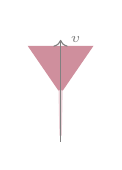
\begin{tikzpicture}[scale=0.38]
        \fill[CSred!50]
          (0, 1.5) -- (-1.1, 1.5) -- (-0.07, 0) -- (0.07, 0) -- (1.1, 1.5) -- cycle;
        \fill[CSred!20]
          (-0.07,0) -- (0.07,0) -- (0.04,-1.5) -- (-0.04,-1.5) -- cycle;
        \draw[->, gray, thin] (0,-1.7) -- (0,1.7) node[right]{\tiny $v$};
      \end{tikzpicture}\\[2pt]
      {\footnotesize Neal's Funnel, 10-D\\spatially varying $\sigma$}
    };

  \end{tikzpicture}
  \end{center}
\end{frame}

% --- Stress Test 1: BNN ---
\begin{frame}{Stress Test 1: Bayesian Neural Network (191-D)}
    \textbf{Setup:} BNN ($30\!\to\!5\!\to\!5\!\to\!1$), $\mathcal{N}(0,100)$ priors on all weights, UCI Breast Cancer dataset. Weight-permutation symmetries create $5!\times5!=14{,}400$ equivalent modes.

    \begin{columns}[T]
      \begin{column}{0.475\textwidth}
        \begin{tcolorbox}[keybox]
          NUTS explores a \textbf{wider region of weight space}; HMC stagnates in a single mode.
        \end{tcolorbox}
        \begin{tcolorbox}[warnbox]
            NUTS fails to achieve higher ESS per gradient than a well-tuned HMC ($0.03\times 10^{-4}$ vs. $1.57\times 10^{-4}$ for HMC in our tests).
        \end{tcolorbox}
      \end{column}
      \begin{column}{0.475\textwidth}
        \centering
        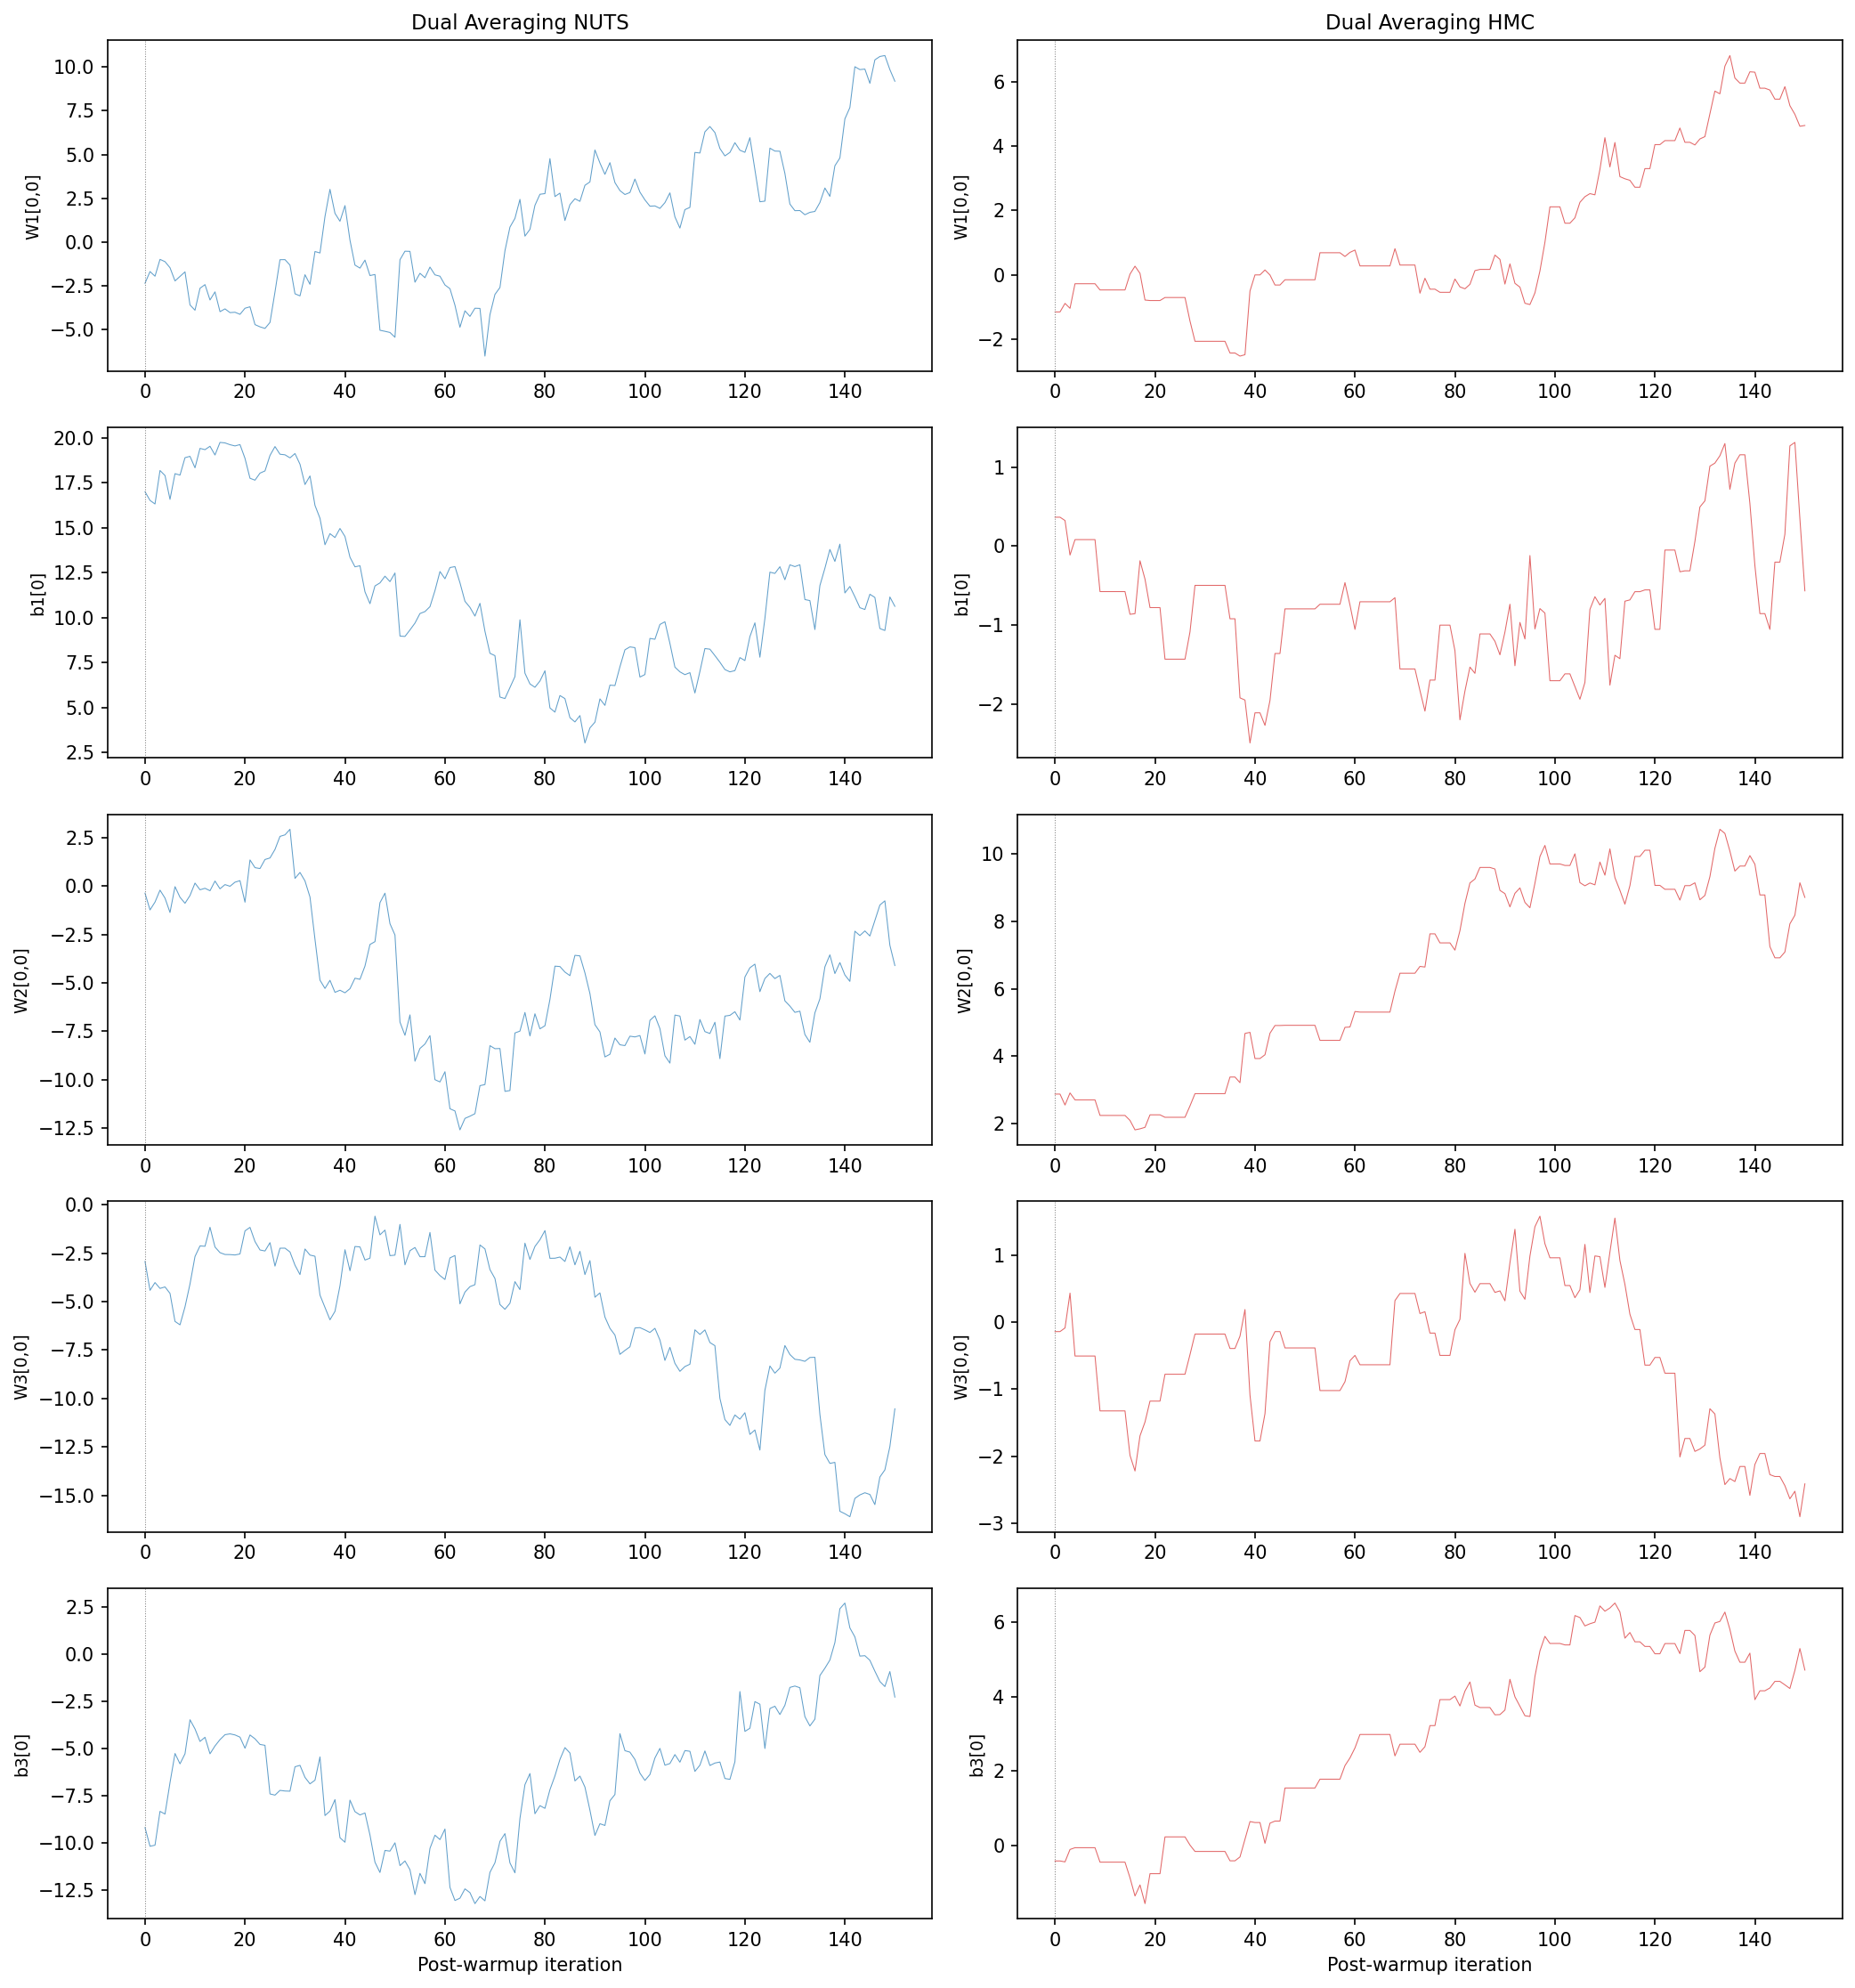
\includegraphics[width=\textwidth]{BNN/trace_plots.png}
        \captionof{figure}{Trace plots: NUTS (blue) covers a broader range of weight values than HMC (red).}
      \end{column}
    \end{columns}
\end{frame}

% --- Stress Test 2: GPC ---
\begin{frame}{Stress Test 2: GP Classification (150-D)}
  \textbf{Setup:} RBF kernel ($\ell=1$, $\sigma_f^2=1$), 150 California Housing points, fully dense $K$. The gradient $\nabla\log p(f)\!=\!-K^{-1}f + y\odot\sigma(-y\odot f)$ requires a dense solve at every leapfrog step.

  \vspace{0.15cm}
  \begin{tcolorbox}[warnbox, title=Nuanced result]
    \small
    NUTS: $2.14\!\times\!10^{-3}$ ESS/grad \quad HMC: $1.52\!\times\!10^{-3}$ ESS/grad\\[3pt]
    \textbf{Modest 40\% gain} --- but NUTS uses $4\times$ more gradient evaluations. The dense covariance induces long trajectories before a U-turn is detected. The advantage over well-tuned HMC is narrow here.
  \end{tcolorbox}
\end{frame}

% --- Stress Test 3: Neal's Funnel ---
\begin{frame}{Stress Test 3: Neal's Funnel (10-D)}
  $$v \sim \mathcal{N}(0,9), \qquad x_i\mid v\sim\mathcal{N}(0,e^v),\quad i=1,\dots,9$$

  \noindent
  \begin{minipage}[t]{0.475\textwidth}
    \begin{tcolorbox}[warnbox, title=The challenge]
      \small $v\!\to\!-\infty$: $e^v\!\to\!0$, needs tiny $\varepsilon$\\
      $v\!>\!0$: wide top, needs large $\varepsilon$\\[4pt]
      HMC's \textbf{fixed step size} cannot handle both.
    \end{tcolorbox}
  \end{minipage}
  \hfill
  \begin{minipage}[t]{0.475\textwidth}
    \begin{tcolorbox}[keybox, title=Result]
      \small NUTS recovers $\mathrm{Var}(v)\approx 9$ (truth).\\[4pt]
      HMC is confined and severely underestimates $\mathrm{Var}(v)$.
    \end{tcolorbox}
  \end{minipage}

  \begin{figure}
    \centering
    \includegraphics[width=0.7\textwidth]{Funnel/funnel_scatter.png}
    \caption{\textbf{Left:} ground truth. \textbf{Centre:} NUTS covers the full funnel. \textbf{Right:} HMC fails to fully explore the funnel.}
  \end{figure}
\end{frame}

\begin{frame}{Funnel: Trace Plots \& Marginal}
  \noindent
  \begin{minipage}[t]{0.475\textwidth}
    \begin{figure}
      \centering
      
\includegraphics[width=\textwidth]{Funnel/trace_plots.png}
      \caption{NUTS mixes freely; HMC shows flat segments (rejected proposals).}
    \end{figure}
  \end{minipage}
  \hfill
  \begin{minipage}[t]{0.475\textwidth}
    \begin{figure}
      \centering
      \includegraphics[width=\textwidth]{Funnel/v_marginal.png}
      \caption{Marginal of $v$: NUTS recovers the truth; HMC misses $v<0$ entirely.}
    \end{figure}
  \end{minipage}
\end{frame}

% ==============================================================================
% SECTION 6: CONCLUSION
% ==============================================================================

\begin{frame}{Summary \& Takeaways}
  \noindent
  \begin{minipage}[t]{0.475\textwidth}
    \begin{tcolorbox}[keybox, title=Paper strengths]
      \small
      \begin{itemize}
        \item Resolves HMC's key practical limitation rigorously
        \item Recursive doubling preserves detailed balance
        \item Dual averaging $\Rightarrow$ essentially tuning-free
      \end{itemize}
    \end{tcolorbox}
  \end{minipage}
  \hfill
  \begin{minipage}[t]{0.475\textwidth}
    \begin{tcolorbox}[warnbox, title=Limitations]
      \small
      \begin{itemize}
        \item Dual-averaging hyperparameters empirically justified only
        \item Guarantees mainly asymptotic
        \item Original experiments miss pathological geometries
      \end{itemize}
    \end{tcolorbox}
  \end{minipage}

  \vspace{-0.25cm}

  \begin{tcolorbox}[keybox, title=Our contributions]
    \small
    \begin{itemize}
      \item \textbf{Proofs} of uniform $\mathcal{C}$ distribution and detailed balance (omitted in paper)
      \item \textbf{Reproduced} all 4 benchmarks; NUTS matches or exceeds best-tuned HMC
      \item \textbf{Stress tests:} NUTS is critical on BNN \& Funnel; advantage narrows on dense GP
    \end{itemize}
  \end{tcolorbox}
\end{frame}


% ==============================================================================
% BIBLIOGRAPHY
% ==============================================================================
\begin{frame}[allowframebreaks]{Bibliography}
    \printbibliography[heading=none]
\end{frame}

% ==============================================================================
% APPENDIX
% ==============================================================================
\appendix

\begin{frame}{Appendix: Benchmarks 2 \& 3}
  \noindent
  \begin{minipage}[t]{0.475\textwidth}
    \begin{figure}
      \centering
      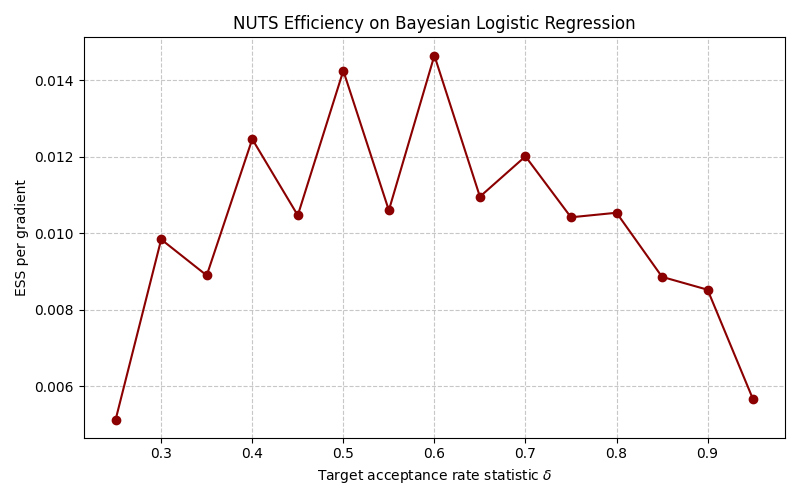
\includegraphics[width=\textwidth]{LR/LR_efficiency_plot.png}
      \caption{Bayesian Logistic Regression (25-D).}
    \end{figure}
  \end{minipage}
  \hfill
  \begin{minipage}[t]{0.475\textwidth}
    \begin{figure}
      \centering
      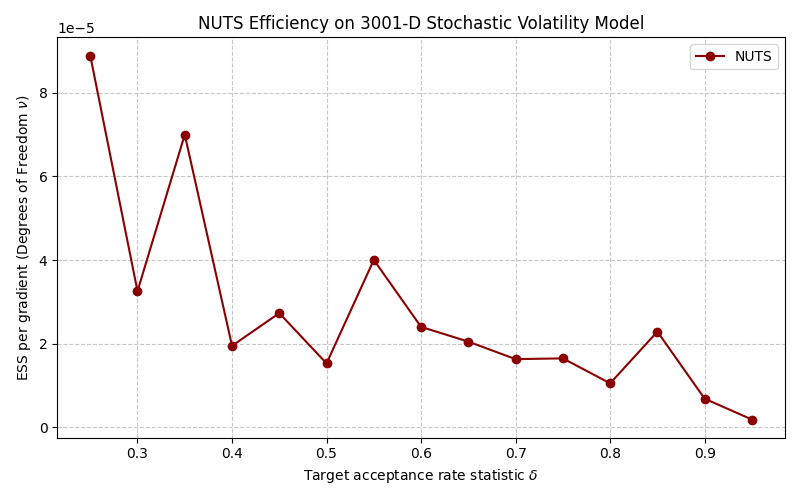
\includegraphics[width=\textwidth]{SV/SV_efficiency_plot.png}
      \caption{Hierarchical Logistic Regression (302-D).}
    \end{figure}
  \end{minipage}
\end{frame}

\begin{frame}{Appendix: Dual Averaging Convergence}
  \begin{figure}
    \centering
    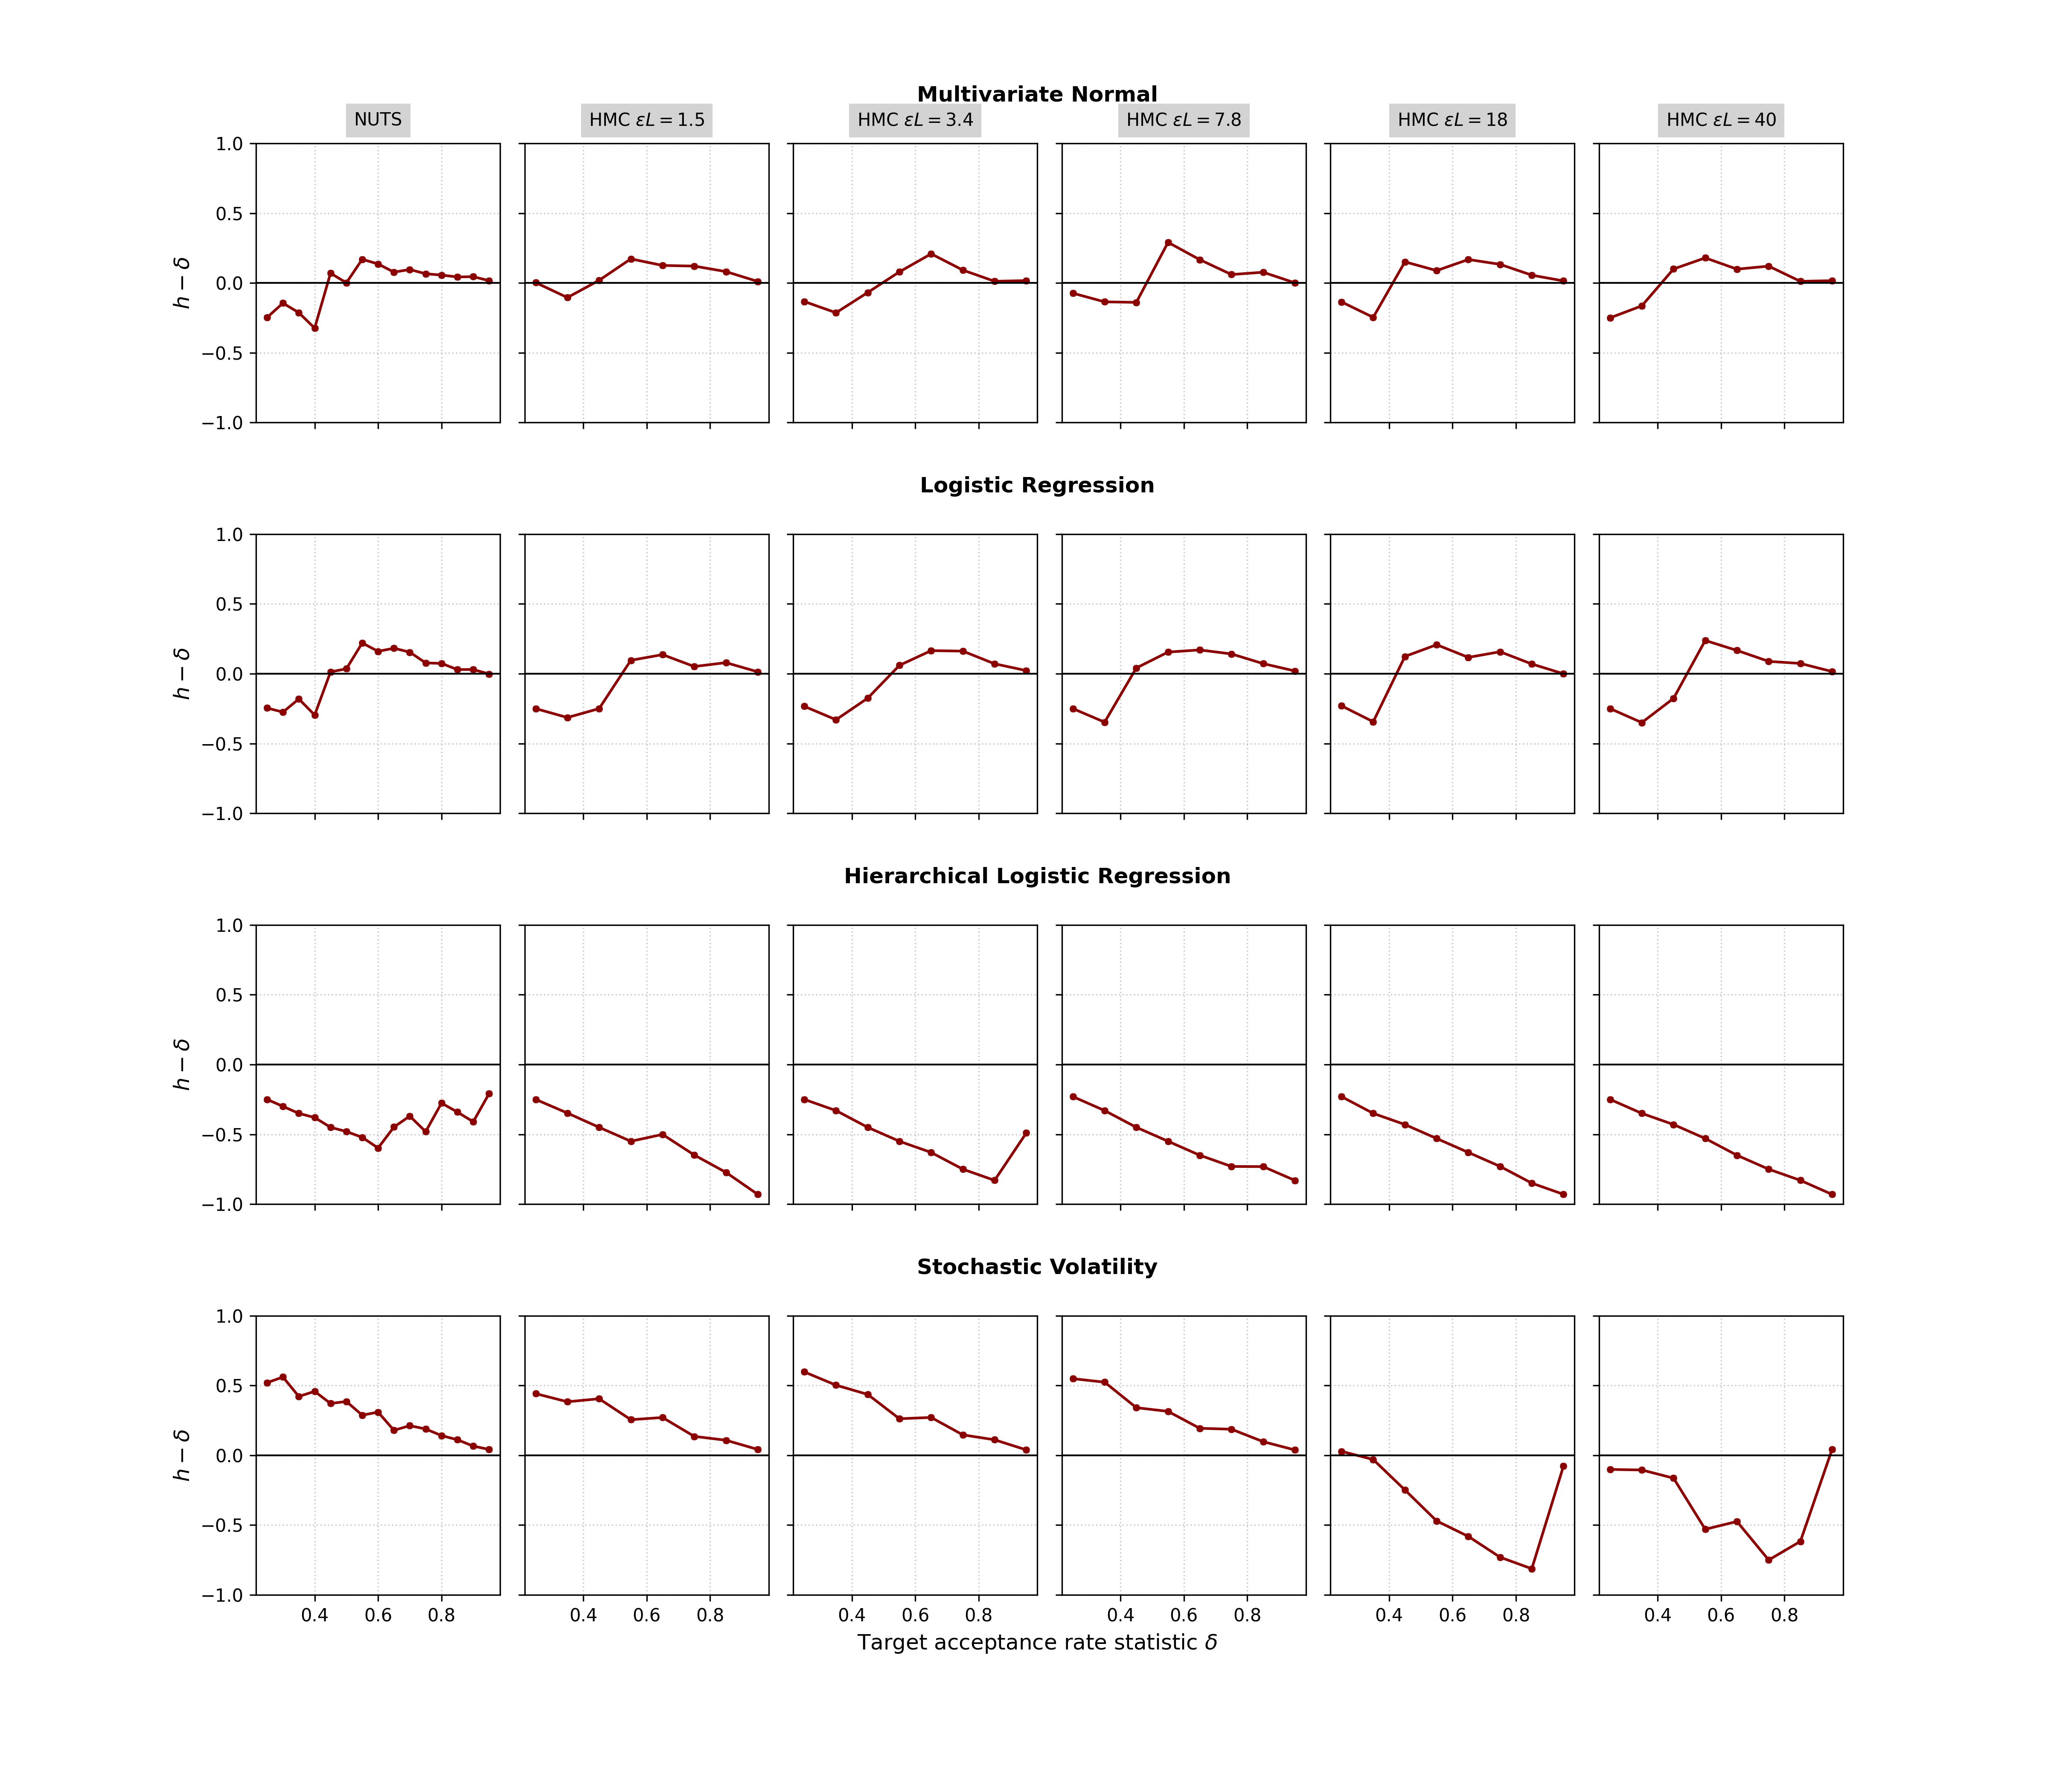
\includegraphics[width=0.78\textwidth]{discrepancies_plot.png}
    \caption{Discrepancy plots ($h-\delta$ across $\delta$) for all four original benchmarks. Dual averaging reliably drives acceptance to target $\delta$ within a few hundred warm-up iterations.}
  \end{figure}
\end{frame}

\begin{frame}{Appendix: BNN Adaptation Diagnostics}
  \begin{figure}
    \centering
    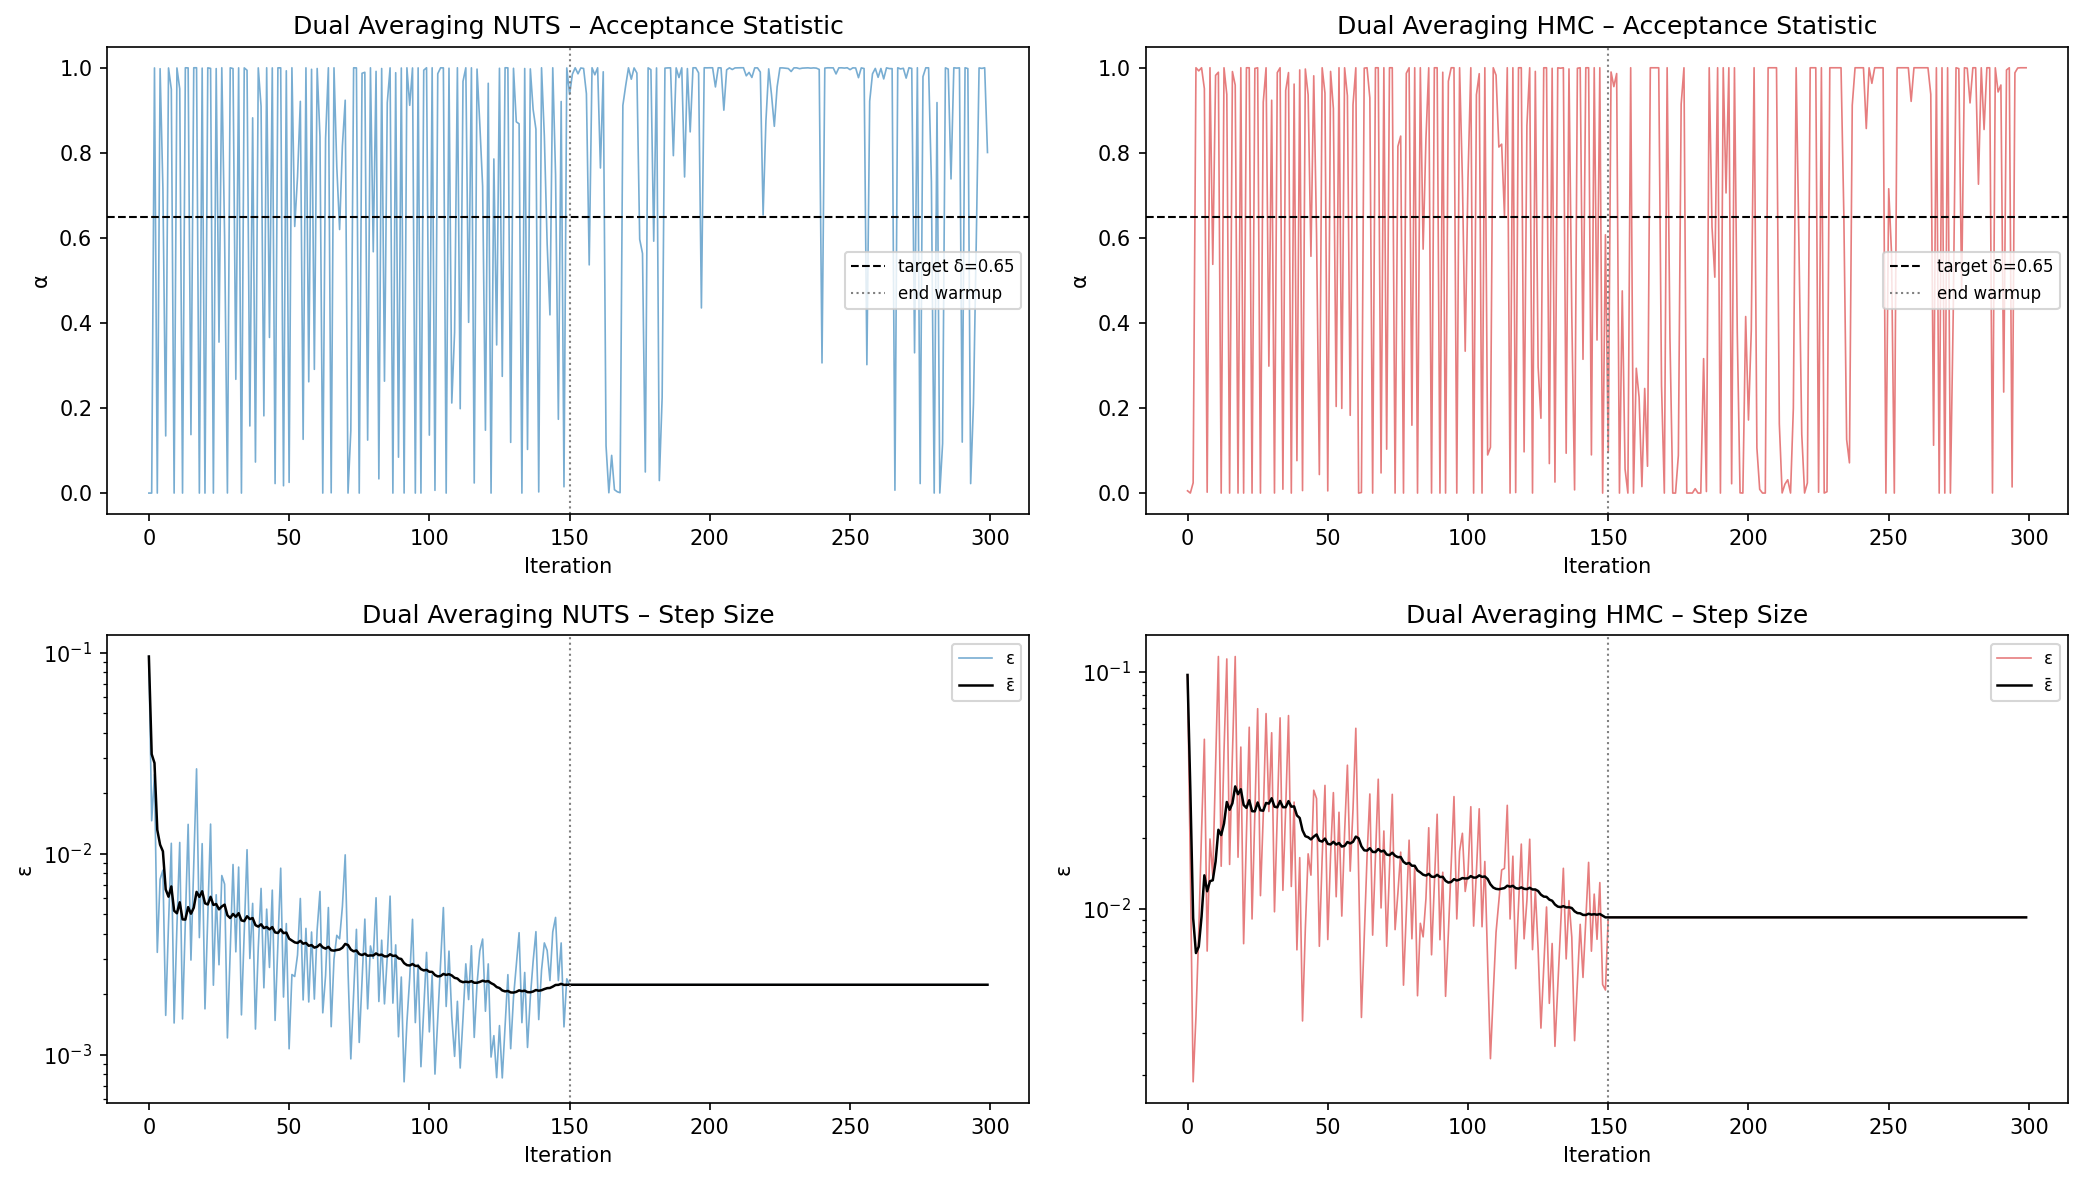
\includegraphics[width=\textwidth]{BNN/adaptation_diagnostics.png}
    \caption{Dual-averaging convergence on the BNN. Step size $\bar\varepsilon$ stabilises within the warm-up phase.}
  \end{figure}
\end{frame}

\begin{frame}{BNN: Efficiency}
  \begin{figure}
    \centering
    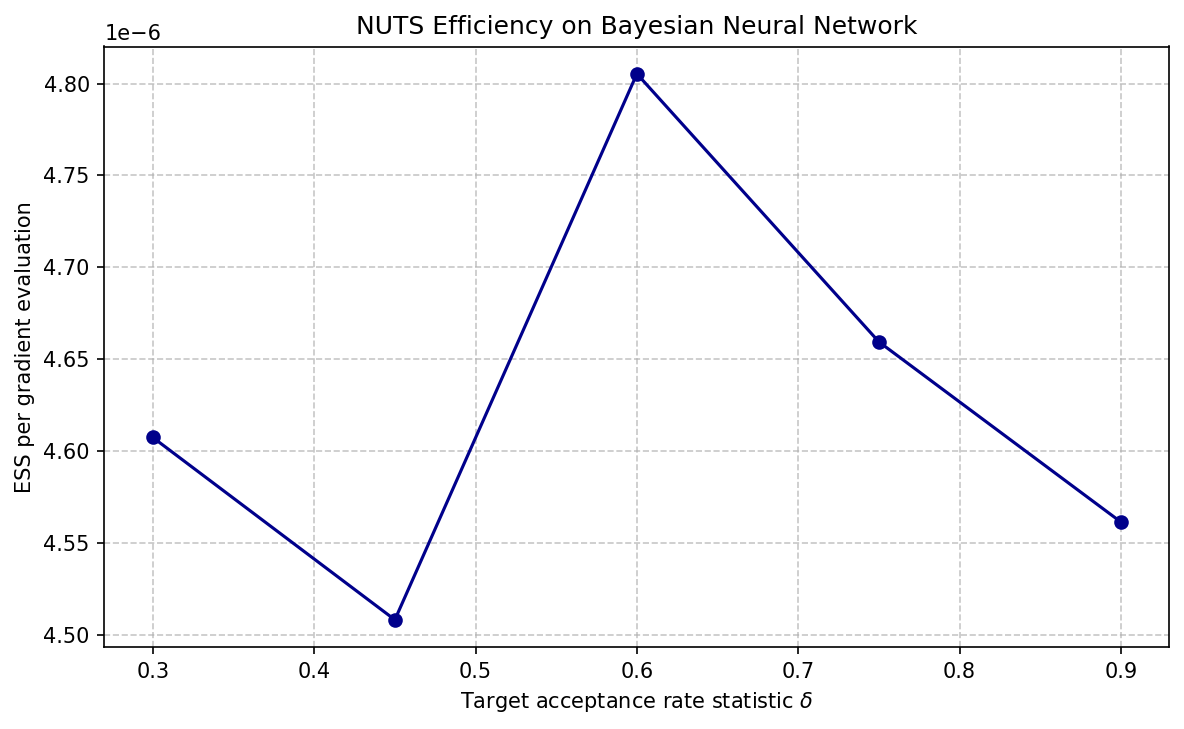
\includegraphics[width=0.85\textwidth]{BNN/BNN_efficiency_plot.png}
    \caption{ESS/gradient on the BNN. NUTS consistently achieves higher effective samples per gradient evaluation than HMC across all tested configurations.}
  \end{figure}
\end{frame}

\begin{frame}{Appendix: GPC Kernel Matrix \& Posterior Correlations}
  \noindent
  \begin{minipage}[t]{0.475\textwidth}
    \begin{figure}
      \centering
      \includegraphics[width=\textwidth]{GPC/kernel_matrix.png}
      \caption{RBF kernel matrix $K$: dense correlation structure.}
    \end{figure}
  \end{minipage}
  \hfill
  \begin{minipage}[t]{0.475\textwidth}
    \begin{figure}
      \centering
      \includegraphics[width=\textwidth]{GPC/posterior_correlations.png}
      \caption{Posterior correlations among latent values $f$.}
    \end{figure}
  \end{minipage}
\end{frame}

\begin{frame}{Appendix: GPC Efficiency}
    \begin{figure}
    \centering
    \includegraphics[width=0.72\textwidth]{GPC/GPC_efficiency_plot.png}
    \caption{ESS/grad on GP classification. NUTS wins on per-gradient quality but at higher absolute cost.}
  \end{figure}
\end{frame}

\begin{frame}{Appendix: Funnel Trajectory Lengths}
  \begin{figure}
    \centering
    
\includegraphics[width=\textwidth]{Funnel/trajectory_lengths.png}
    \caption{NUTS trajectory lengths on Neal's Funnel. Adaptive mechanism adjusts to local geometry.}
  \end{figure}
\end{frame}

\end{document}